\documentclass{beamer}

% IMAGENES UTILIZADAS
% https://www.flickr.com/photos/13166455@N05/6902172784/sizes/o/in/photostream/
% https://www.flickr.com/photos/13166455@N05/9026747558/
% http://www.freepik.com/index.php?goto=74&idfoto=778705
% http://www.freepik.com/free-icon/mp3-audio-file_740342.htm#term=mp3&page=1&position=0
%   Icon made by [http://www.freepik.com]Freepik from [http://www.flaticon.com]www.flaticon.com
%   licensed under [http://creativecommons.org/licenses/by/3.0/]CC BY 3.0
% http://getlevelten.com/blog/ian-whitcomb/whats-wrong-project-application-queue
% http://butdoesitfloat.com/I-hoped-for-nothing-And-yet-I-lived-in-expectation

\mode<presentation> {\usetheme{Berkeley}\setbeamertemplate{navigation symbols}{}}

\usepackage[T1]{fontenc}
\usepackage[utf8]{inputenc}
\usepackage[spanish]{babel}
\usepackage{graphicx}
\usepackage{booktabs}
\usepackage{lmodern}
\usepackage{cite}
\usepackage{hyperref}
\usepackage{url}
\usepackage{tikz}
\usepackage{color}

\definecolor{commonBg}{RGB}{180,150,60}
\definecolor{gris}{RGB}{140,140,140}

\setbeamercolor{title}{fg=white, bg=}
\setbeamercolor{subtitle}{fg=white, bg=}
\setbeamercolor{author}{fg=white, bg=}
\setbeamercolor{institute}{fg=white, bg=}
\setbeamercolor{date}{fg=white, bg=}
\setbeamercolor{title in sidebar}{fg=white, bg=}
\setbeamercolor{author in sidebar}{fg=white, bg=}
\setbeamercolor{section in toc}{fg=white}
\setbeamercolor{subsection in toc}{fg=white}
\setbeamercolor{background canvas}{bg=white}
\setbeamercolor{block title}{bg=commonBg}
\setbeamercolor{block body}{bg=white}
\setbeamercolor{headline}{bg=commonBg}
\setbeamercolor{sidebar}{bg=commonBg}
\setbeamercolor{section in sidebar}{bg=white,fg=commonBg}
\setbeamercolor{structure}{bg=commonBg, fg=commonBg}

\usebackgroundtemplate{\tikz\node[opacity=0.08]{\includegraphics[height=\paperheight,width=\paperwidth]{Recursos/cloud2.jpg}};}

\title[Priority Queue]{\huge{Priority Queue}\\\small{\textit{Cola con Prioridad}}}
\author{Emilio Rojas}
\institute[DSA]
{
    Estructuras Abstractas de Datos y Algorítmos para Ingeniería\\
    \medskip
    \small{\textit{emilio93@gmail.com}}
}
\date{\today}

\begin{document}
\nocite{knuth1973the}
\nocite{weiss2013estructuras}
\nocite{wiki:Multiset}
\nocite{wiki:set}
\nocite{MultisetasAntiset}
\nocite{rucker1995infinity}
\nocite{kolman1997estructuras}
\nocite{blizard1988}
\nocite{1_msdn.microsoft.com_2015}
\nocite{wiki:rbtree}

%******************************%
% CONTENIDO DE LA PRESENTACIÓN %
%******************************%
%\section{Portada}

    {
    \usebackgroundtemplate{\tikz\node[opacity=0.85]{ 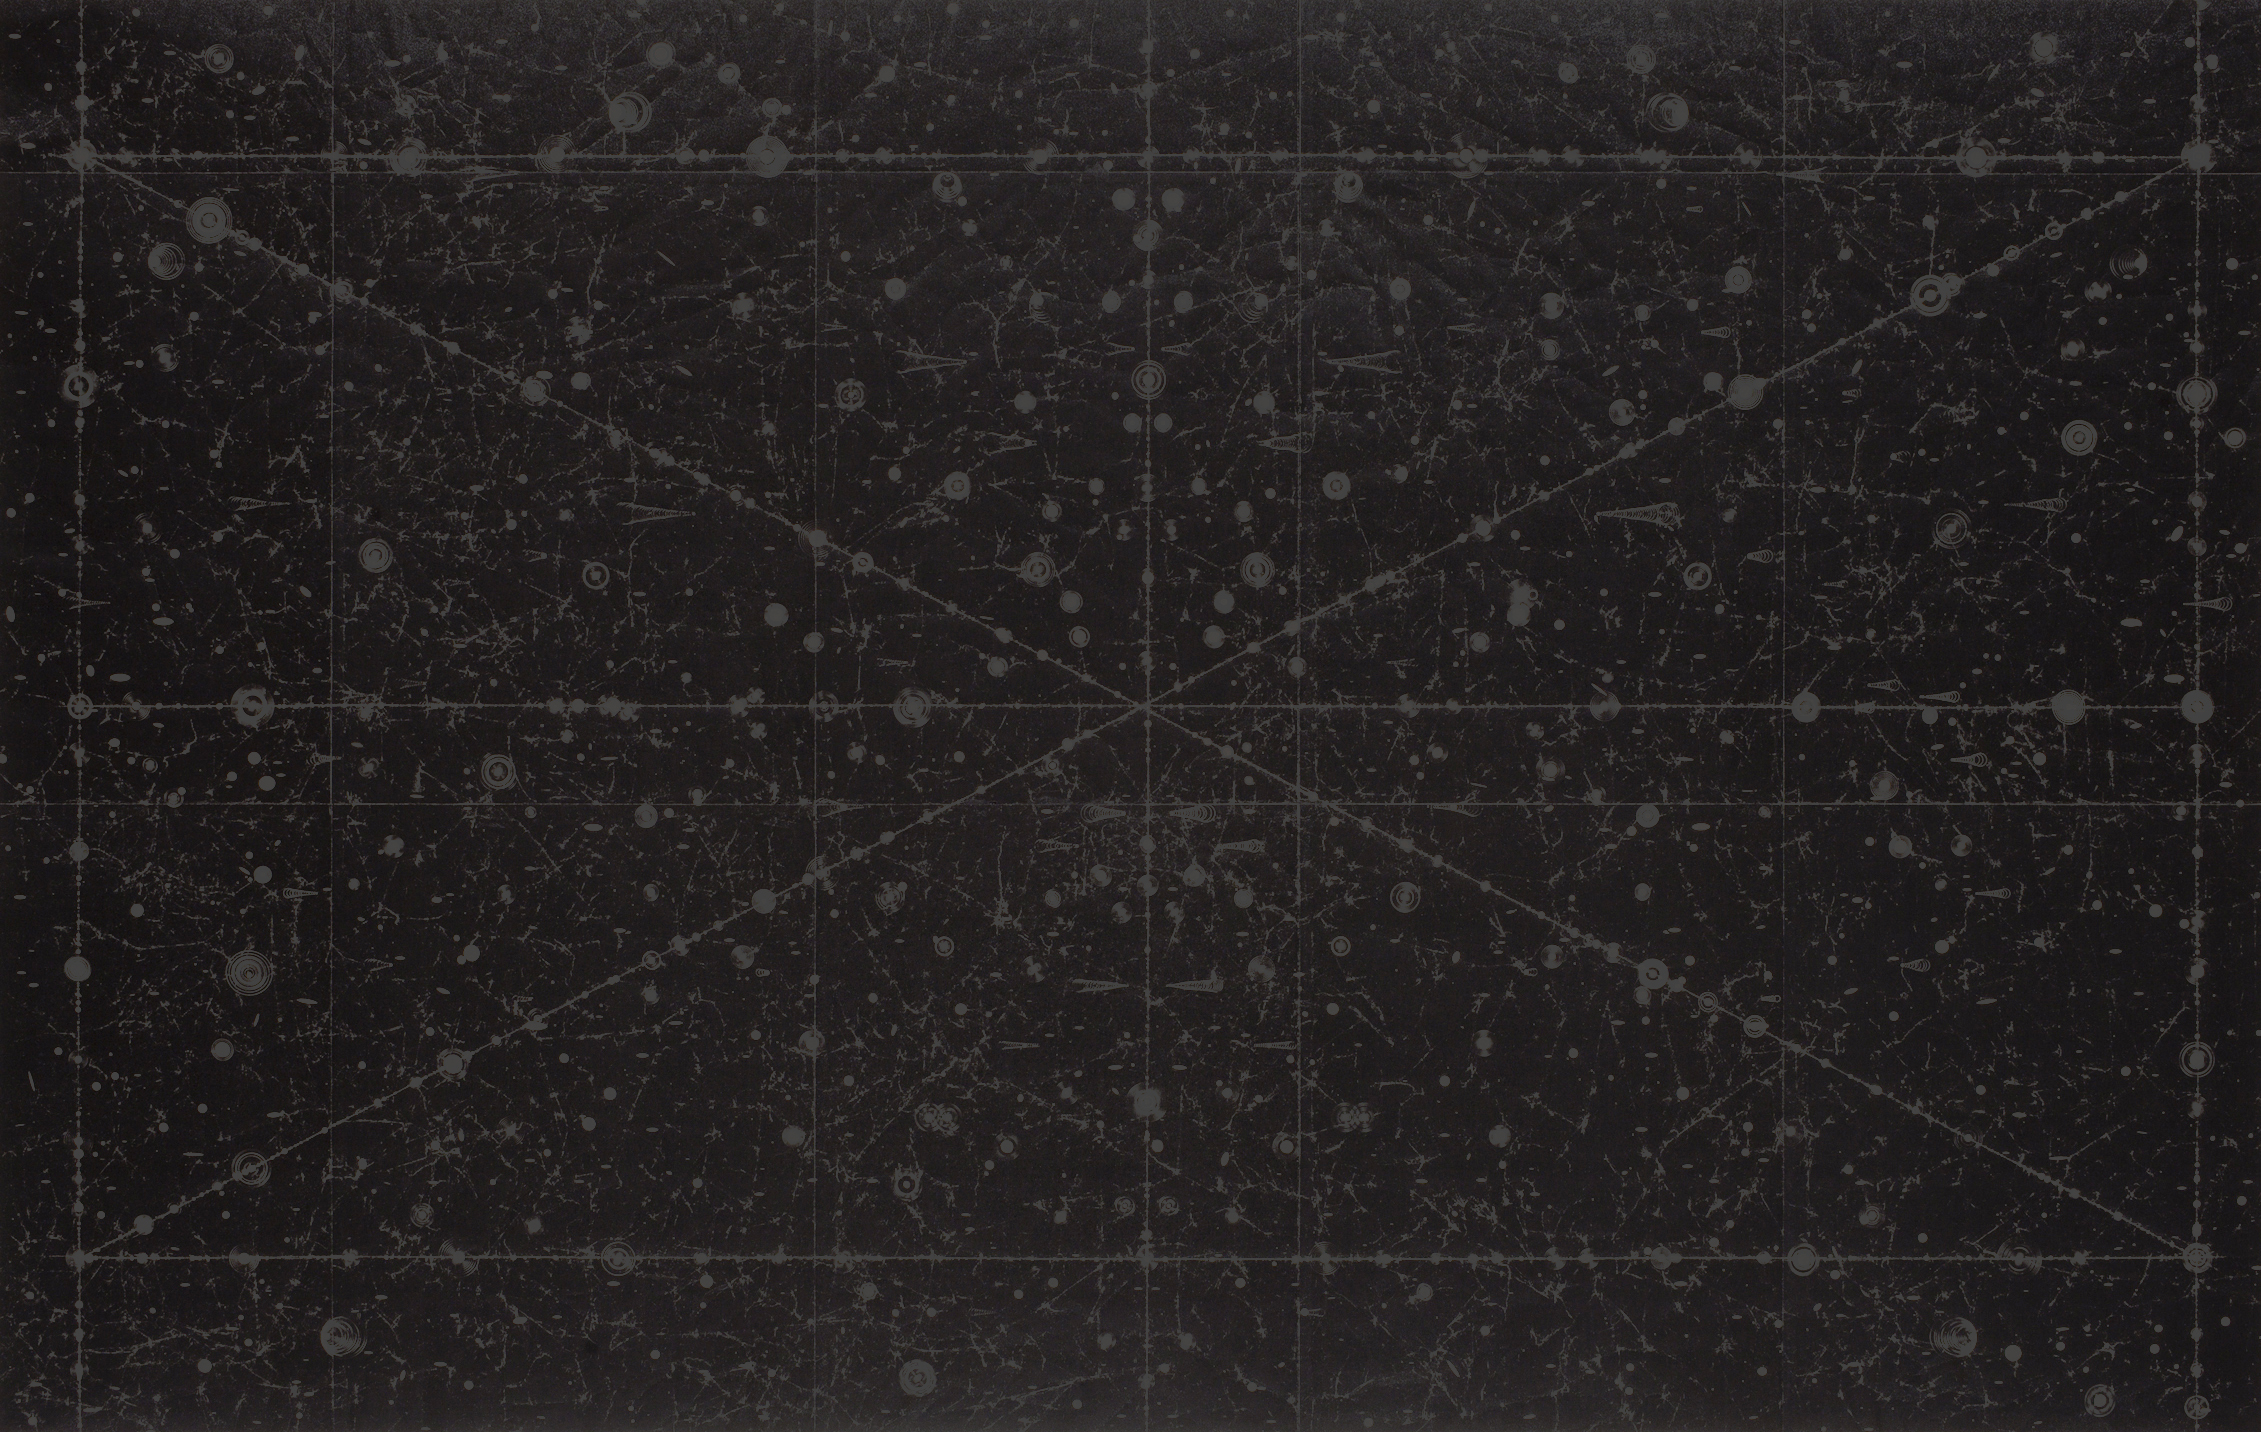
\includegraphics[height=\paperheight,width=\paperwidth]{Recursos/otto.jpg}};}
    \begin{frame}
        \titlepage
        %\begin{center}
        %    \huge{Sets, Multisets y Hashs}\\
        %    Emilio Rojas\\
        %    Estructuras Abstractas de Datos y algoritmos para Inegiería\\
        %\end{center}
    \end{frame}
    }

%\section{Contenido}

%    {
%    \usebackgroundtemplate{\tikz\node[opacity=0.85]{ 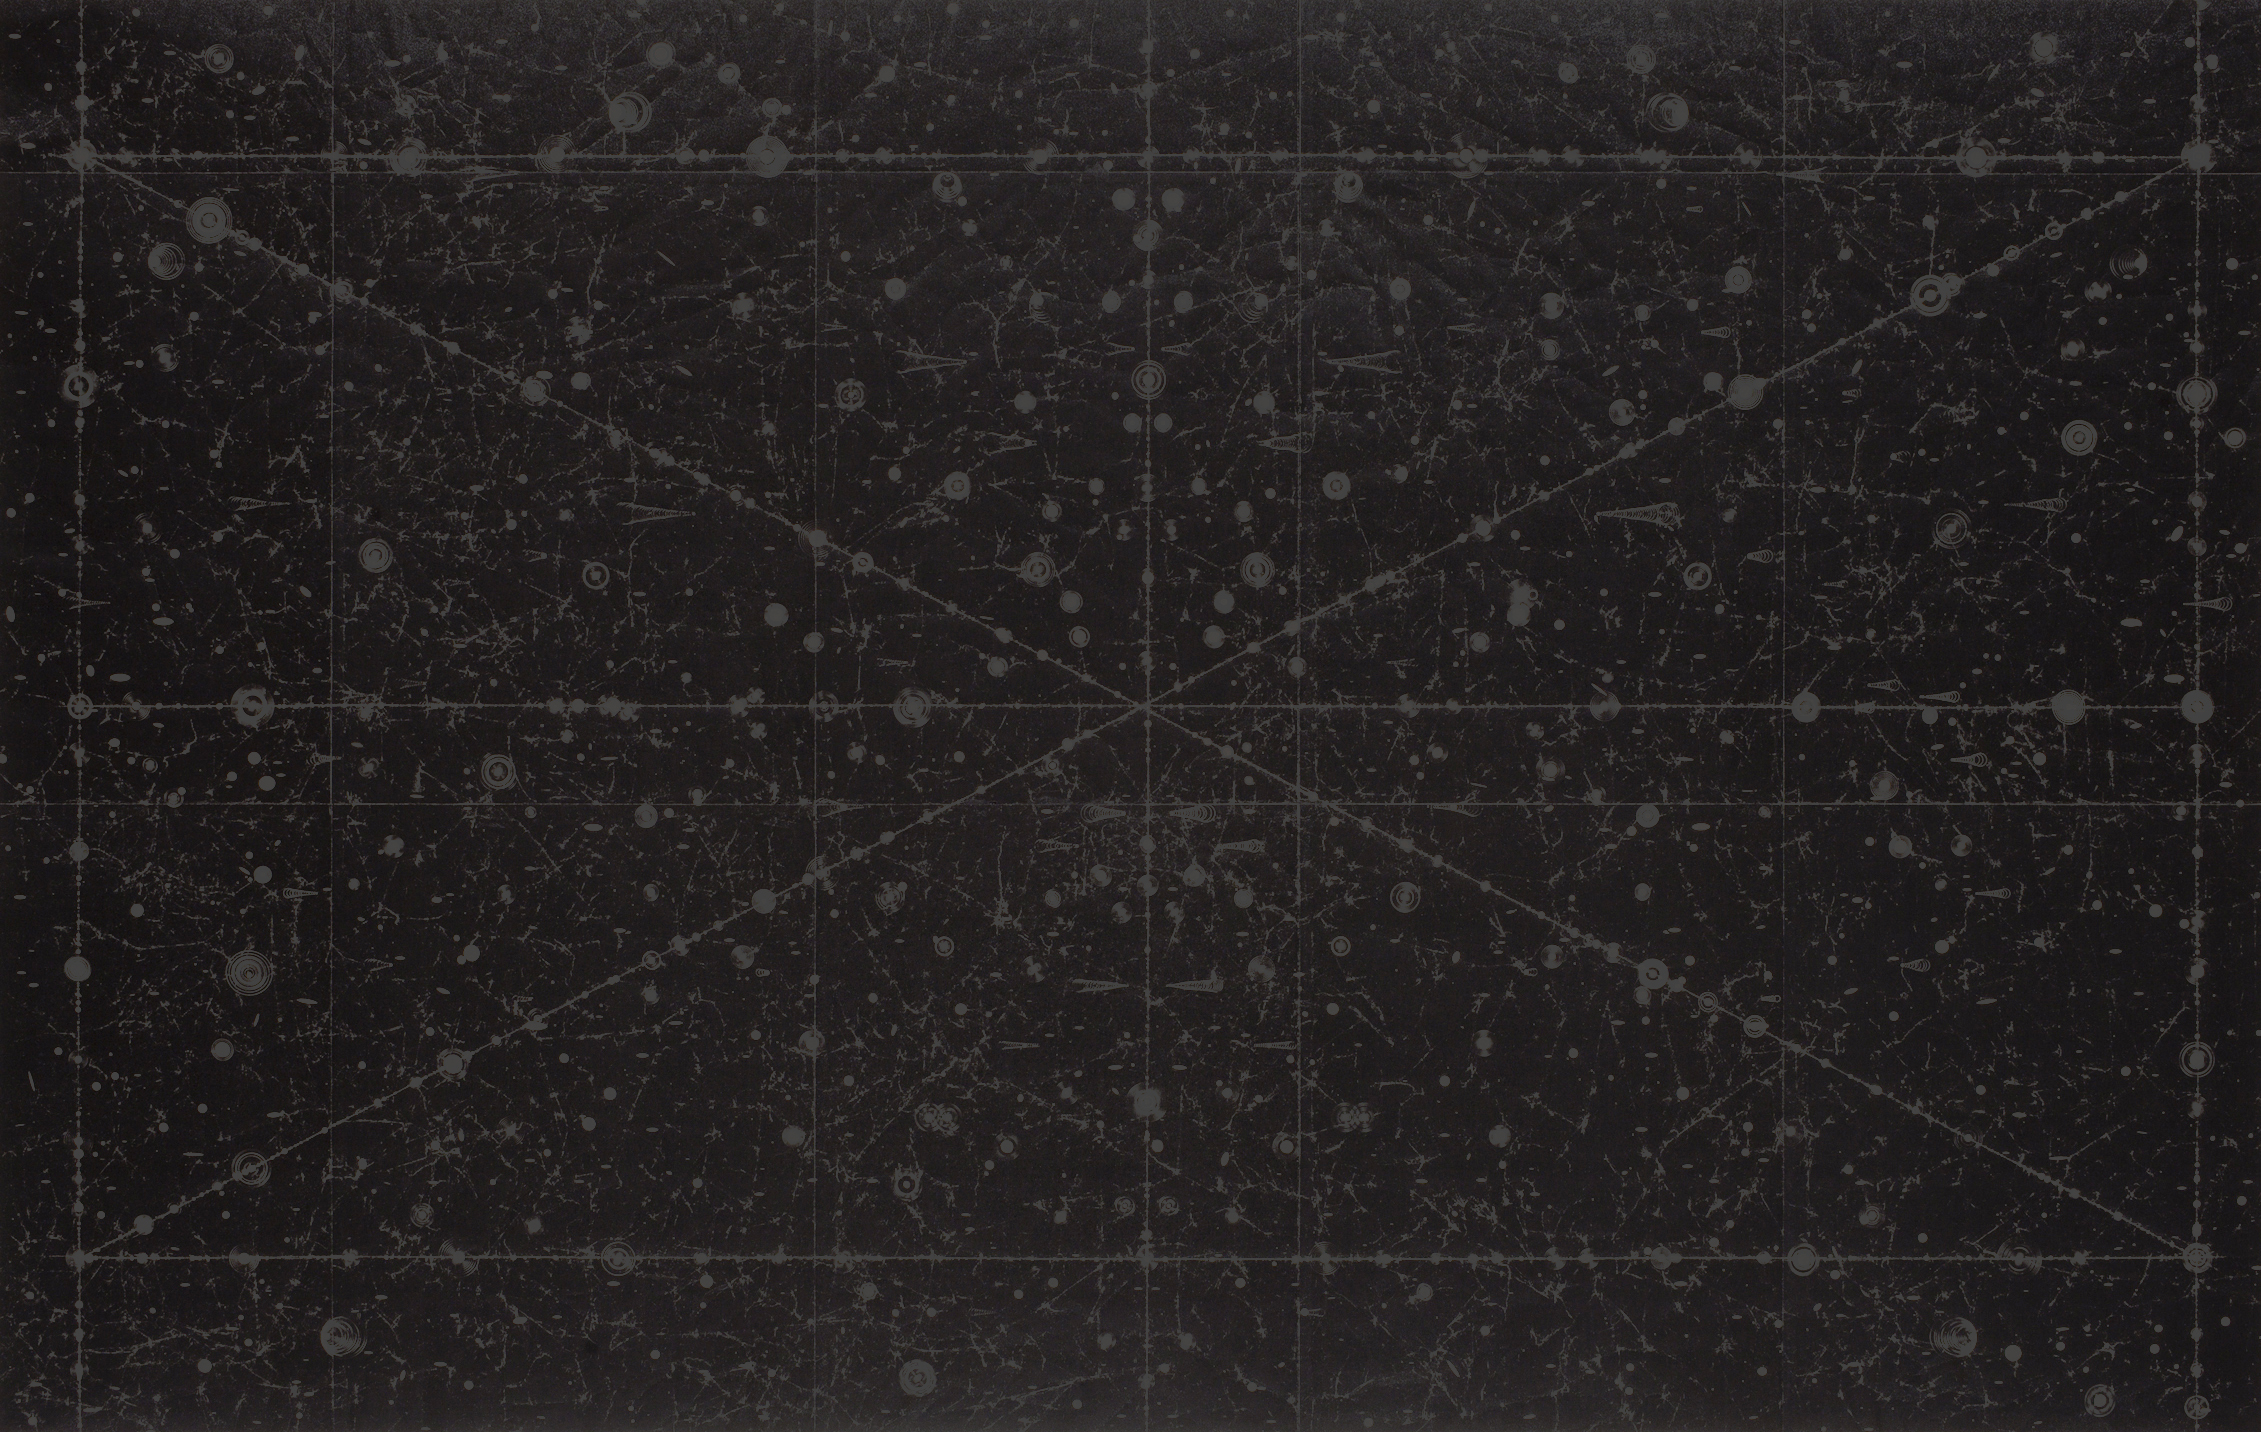
\includegraphics[height=\paperheight,width=\paperwidth]{Recursos/otto.jpg}};}
%    \begin{frame}
%        \frametitle{Contenido}
%        \color{white}
%        \tableofcontents
%    \end{frame}
%    }

\section{¿Porque?}

    \begin{frame}
        \frametitle{¿Porque?}
        \begin{itemize}
            \item Una cola con prioridad es una generalización de una fila.
            \item Mejor organización de una serie de elementos para su procesamiento.
        \end{itemize}
        \begin{center}
            
\includegraphics[width=0.5\textwidth]{Recursos/kindaQueue.jpg}
        \end{center}
        \pause
    \end{frame}

    \begin{frame}
        \frametitle{¿Donde lo puedo usar?}
        \begin{itemize}
            \item Simulación de eventos
            \begin{itemize}
                \item Fila en banco para adulto/as, embarazadas, discapacitado/as, etc.
                \item Inventario de un supermercado
            \end{itemize}

            \item Compresión de datos(Codificación Huffman)
            % <<En ciencias de la computación y teoría de la información, la
            % codificación Huffman es un algoritmo usado para compresión de
            % datos. El término se refiere al uso de una tabla de códigos de
            % longitud variable para codificar un determinado símbolo (como
            % puede ser un carácter en un archivo), donde la tabla ha sido
            % rellenada de una manera específica basándose en la probabilidad
            % estimada de aparición de cada posible valor de dicho símbolo.>>
            % https://es.wikipedia.org/wiki/Codificaci%C3%B3n_Huffman

            \item Graph searching. (Dijkstra's algorithm)
            % Prim's algorithm
            % http://www.cs.bris.ac.uk/~montanar/teaching/dsa/dijkstra-handout.pdf

            \item ..., Inteligencia artificial, SO, Filtros de Spam, ...
            % https://www.cs.princeton.edu/~rs/AlgsDS07/06PriorityQueues.pdf

        \end{itemize}
        \begin{center}
            \only<1>{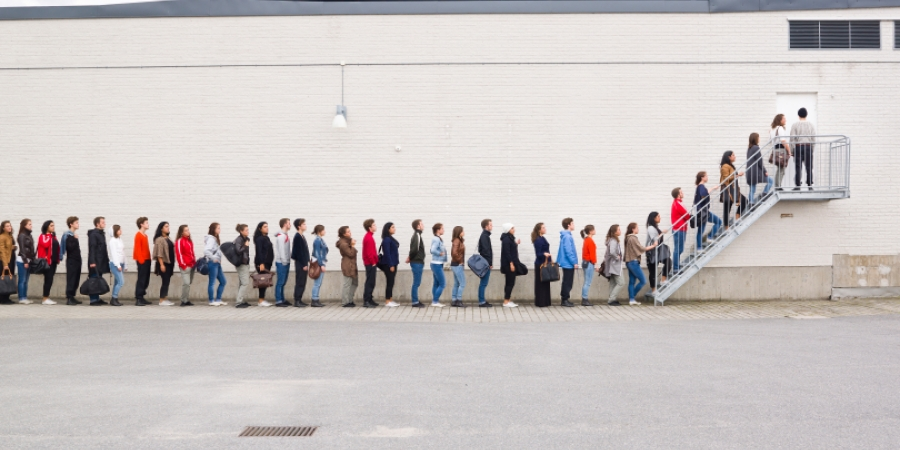
\includegraphics[width=0.25\textwidth]{Recursos/pplQueue.jpg}}
            \only<2>{
\includegraphics[width=0.25\textwidth]{Recursos/mp3.pdf}}
        \end{center}
    \end{frame}

\section{}

    \begin{frame}
        \frametitle{Fin}
        \centering
        \Huge{Gracias}\\
        \small{Preguntas, Comentarios}
        %\vfill
        %\hfill \tiny{\textit{A story has no beginning or end: arbitrarily one chooses that moment of experience from which to look back or from which to look ahead.\\}}
        %\hfill \tiny{G. Greene}

    \end{frame}

%No se utiliza para la presentacion
%\section{Referencias}
%{\usebackgroundtemplate{\tikz\node[opacity=0.35]{ \includegraphics[height=\paperheight,width=\paperwidth]{Recursos/pia.jpg}};}
%\begin{frame}[allowframebreaks]\frametitle{Referencias}\bibliographystyle{alpha}\bibliography{refs}\end{frame}}


\end{document}
